\documentclass[conference]{IEEEtran}
\IEEEoverridecommandlockouts
\usepackage{cite}
\usepackage{amsmath,amssymb,amsfonts}
\usepackage{algorithmic}
\usepackage{graphicx}
\usepackage{textcomp}
\usepackage{xcolor}
\usepackage{booktabs}
\usepackage{multirow}
\usepackage{url}

\def\BibTeX{{\rm B\kern-.05em{\sc i\kern-.025em b}\kern-.08em
    T\kern-.1667em\lower.7ex\hbox{E}\kern-.125emX}}

\begin{document}

\title{Green-Surrogate Assisted Multi-Objective Optimization and Multivariate Fault Monitoring of a Coastal Hybrid Wind--Solar--PEM Green Hydrogen Plant under Meteorological Uncertainty}

\author{\IEEEauthorblockN{Krishnendu}
\IEEEauthorblockA{\textit{Department of Computer Science and Engineering} \\
\textit{Manipal Institute of Technology (MIT)}\\
\textit{Manipal Academy of Higher Education (MAHE)}\\
Manipal, Karnataka 576104, India}
\and
\IEEEauthorblockN{Arav Aggarwal}
\IEEEauthorblockA{\textit{Department of Civil Engineering, School of Civil \& Chemical Engineering} \\
\textit{Manipal Institute of Technology (MIT)}\\
\textit{Manipal Academy of Higher Education (MAHE)}\\
Manipal, Karnataka 576104, India}
}

\maketitle

\begin{abstract}
Industrial decarbonization of coastal refining, fertilizer, and specialty chemical clusters in India demands uninterrupted, cost-effective green hydrogen ($\text{H}_2$) generation under stochastic meteorological forcing and coastal site constraints. Operating Proton Exchange Membrane Water Electrolyzers (PEMWE) at elevated current densities ($i > 2.0\text{ A/cm}^2$) offers substantial capital cost reductions by maximizing $\text{H}_2$ flux per unit active membrane area, yet introduces severe nonlinear trade-offs between two-phase mass-transport overpotential, dynamic voltage degradation, and membrane-electrode assembly (MEA) fault vulnerability. In this study, we develop a unified Process Systems Engineering (PSE) and Green Artificial Intelligence framework combining coastal civil/wind-resource siting, first-principles high-current-density PEMWE modeling, physics-informed \textbf{Green Deep Learning} surrogate optimization, Explainable AI (XAI), and Principal Component Analysis (PCA) multivariate fault monitoring for a $500\text{ kg H}_2/\text{h}$ ($4,380\text{ t/yr}$) hybrid Wind--Solar--Battery--PEMWE facility in the Manipal--Mangalore coastal corridor ($13.35^\circ\text{N}, 74.79^\circ\text{E}$). Extending recent high-current PEMWE formulations and distributed wind-to-hydrogen design methodologies, we embed dimensionless electrochemical and dispatch invariants into a lightweight Multi-Layer Perceptron (\textbf{Green-MLP}). Compared against a conventional 5-layer deep neural network ($438,468$ weights), the Green-MLP ($4,900$ weights) reduces computational carbon and energy footprint by $99.38\%$ while improving out-of-sample generalization ($R^2 = 0.9977$ on Levelized Cost of Hydrogen [LCOH], $0.9992$ on supply reliability) and accelerating $8,760$-hour plant evaluations by $10,592\times$. Coupling the Green-MLP with Non-dominated Sorting Genetic Algorithm II (NSGA-II) and exact differential-algebraic equation (DAE) verification yields an optimal Pareto knee-point plant ($51.13\text{ MW}$ coastal wind, $94.73\text{ MW}$ solar PV, $38.98\text{ MW}$ nominal PEM stack operating dynamically up to $i_{\max}^* = 2.84\text{ A/cm}^2$, and $20.07\text{ MWh}$ $\text{LiFePO}_4$ storage) achieving an LCOH of INR $296.70/\text{kg H}_2$ (\$$3.53/\text{kg}$), a Loss of Hydrogen Supply Probability (LPSP) of $0.94\%$, and a stack lifetime of $10.83\text{ years}$---reducing LCOH by $9.79\%$ and $21.60\%$ relative to wind-only and solar-only baselines. Finally, a latent-variable PCA fault monitoring architecture utilizing Hotelling's $T^2$ and Jackson--Mudholkar Squared Prediction Error ($\text{SPE}/Q$) control charts across $10$ coupled process variables detects incipient membrane dehydration $52\text{ hours}$ earlier than univariate voltage alarms ($89.09\%$ fault detection rate on $Q$, $91.82\%$ on $T^2$) and isolates high-current anodic bubble flooding with $100.0\%$ accuracy ($1.86\%$ false alarm rate).
\end{abstract}

\begin{IEEEkeywords}
Explainable AI (XAI), green deep learning, green hydrogen, high-current-density PEM water electrolyzer, multivariate statistical process monitoring (PCA), multi-objective optimization (NSGA-II), wind-to-hydrogen systems.
\end{IEEEkeywords}

\section{Introduction}
\IEEEPARstart{T}{he} National Green Hydrogen Mission of India targets $5\text{ MMT/yr}$ of green hydrogen production capacity by 2030 to decarbonize hard-to-abate petrochemical refineries, ammonia/urea complexes, and steel manufacturing units \cite{mnre2023}. Coastal industrial corridors along the Arabian Sea---specifically the Udupi--Manipal--Mangalore belt in Karnataka hosting Mangalore Refinery and Petrochemicals Limited (MRPL) and Mangalore Chemicals \& Fertilizers (MCF)---offer strategic proximity to industrial hydrogen off-takers, port infrastructure, and abundant renewable resources \cite{pujari2026}. However, standalone solar photovoltaic (PV) or wind-powered electrolysis in tropical coastal monsoon climates faces severe seasonal intermittency: solar global horizontal irradiance (GHI) plunges by over $50\%$ during the four-month Southwest Monsoon (June--September), whereas standalone wind power drops during pre-monsoon summer months (February--May) \cite{mitra2025book, abhishek2025}.

Recent advances at the intersection of chemical process systems, civil-environmental siting, and computational intelligence have highlighted three critical paradigms for overcoming these techno-economic barriers:
\begin{enumerate}
    \item \textit{High-Current-Density PEM Electrolysis and Distributed Hybrid Synthesis:} Masampally, Mitra, and Runkana \cite{masampally2026} recently demonstrated through rigorous electrochemical modeling that operating Proton Exchange Membrane Water Electrolyzers (PEMWE) at elevated current densities ($i \in [2.0, 3.5]\text{ A/cm}^2$) substantially increases hydrogen production per unit active membrane area, thereby slashing stack capital expenditure (CAPEX) per unit capacity. However, high-current operation exacerbates two-phase oxygen/hydrogen bubble crowding within the porous transport layer (PTL), increases ohmic and concentration overpotentials, and accelerates voltage degradation under stochastic wind ramping \cite{carmo2013, liso2018}.
    \item \textit{Physics-Informed ``Green Deep Learning'' Surrogates:} Optimizing hybrid renewable-to-hydrogen plants across $8,760$ hourly meteorological steps over multi-decade lifetimes requires tens of thousands of dynamic differential-algebraic equation (DAE) evaluations during evolutionary search \cite{inapakurthi2025}. Pujari, Inapakurthi, and Mitra \cite{pujari2026} established that replacing computationally wasteful, over-parameterized black-box deep neural networks with compact, physics-guided ``Green Deep Learning'' surrogates enables high-precision multi-objective Pareto design while reducing training energy and carbon footprint by orders of magnitude \cite{schwartz2020, raissi2019}.
    \item \textit{Multivariate Statistical Process Monitoring (MSPM) for Fault-Resilient Operation:} Under volatile monsoon wind gusts and high-current excursions, PEMWE stacks are vulnerable to incipient internal faults, notably cationic fouling/dehydration of the Nafion proton-conducting membrane and anodic PTL mass-transport flooding, which can trigger hazardous $\text{H}_2$-in-$\text{O}_2$ gas crossover if left unmonitored \cite{siracusano2017}. As established in the chemical process monitoring literature by Madakyaru and co-workers \cite{madakyaru2024, nounou2012, qin2012}, univariate threshold alarms on cell voltage or stack temperature fail to detect subtle breakdowns in cross-variable correlations during wide load swings, necessitating latent-variable projection methods such as Principal Component Analysis (PCA) with Hotelling's $T^2$ and Jackson--Mudholkar Squared Prediction Error ($\text{SPE}/Q$) control charts \cite{jackson1979}.
\end{enumerate}

Despite these parallel advances, no prior study has unified (i) real hourly coastal Karnataka monsoon/summer meteorological complementarity and civil terrain wind-shear siting, (ii) first-principles high-current PEMWE modeling up to $3.5\text{ A/cm}^2$ with dynamic ramping degradation, (iii) physics-guided Green Deep Learning surrogate optimization with Explainable AI (XAI) and Monte Carlo financial risk quantification, and (iv) online multivariate PCA $T^2/Q$ fault detection and root-cause isolation within a single cohesive architecture. This paper bridges this gap.

\section{Coastal Infrastructure Siting and First-Principles Electrochemical Modeling}

\subsection{Coastal Karnataka Meteorology and Civil Terrain Wind-Shear Siting}
Hourly meteorological time series for the Manipal--Udupi--Mangalore coastal corridor ($\text{lat} = 13.3525^\circ\text{N}, \text{lon} = 74.7928^\circ\text{E}$) spanning a complete $8,760$-hour reference year were extracted from the NASA POWER Agroclimatology and Renewable Energy archive \cite{nasapower2026}, comprising all-sky surface downward shortwave irradiance ($\text{GHI}$, $\text{W/m}^2$), wind speeds at $10\text{ m}$ and $50\text{ m}$ ($v_{10}, v_{50}$, $\text{m/s}$), and ambient air temperature at $2\text{ m}$ ($T_{\text{amb}}$, $^\circ\text{C}$). Accounting for coastal lateritic plateau roughness and boundary-layer stability, hub-height wind speed at $h_{\text{hub}} = 100\text{ m}$ is evaluated via time-varying power-law wind shear $\alpha(t)$ and calibrated with the National Institute of Wind Energy (NIWE) coastal ridge/nearshore acceleration factor ($f_{\text{coastal}} = 1.58$) \cite{gupta2021}:
\begin{equation}
\alpha(t) = \frac{\ln\big(v_{50}(t)/v_{10}(t)\big)}{\ln(50/10)}, \quad v_{\text{hub}}(t) = f_{\text{coastal}}\, v_{50}(t) \left(\frac{h_{\text{hub}}}{50}\right)^{\alpha(t)}
\label{eq:wind_shear}
\end{equation}

For a Class-IIIA coastal wind turbine ($v_{\text{ci}} = 2.5\text{ m/s}$, $v_r = 8.4\text{ m/s}$, $v_{\text{co}} = 25.0\text{ m/s}$, array wake efficiency $\eta_{\text{array}} = 0.95$) and N-type monocrystalline silicon solar PV arrays with thermal derating ($\gamma_T = -0.38\%/^\circ\text{C}$ above $25^\circ\text{C}$, inverter efficiency $\eta_{\text{inv}} = 0.96$), the instantaneous hourly capacity factors $CF_{\text{wind}}(t)$ and $CF_{\text{solar}}(t)$ are given by:
\begin{equation}
CF_{\text{wind}}(t) = \eta_{\text{array}} \begin{cases} 
0, & v_{\text{hub}}(t) < v_{\text{ci}} \text{ or } v_{\text{hub}}(t) > v_{\text{co}} \\
\dfrac{v_{\text{hub}}(t)^3 - v_{\text{ci}}^3}{v_r^3 - v_{\text{ci}}^3}, & v_{\text{ci}} \le v_{\text{hub}}(t) < v_r \\
1.0, & v_r \le v_{\text{hub}}(t) \le v_{\text{co}}
\end{cases}
\label{eq:cf_wind}
\end{equation}
\begin{equation}
CF_{\text{solar}}(t) = \min\!\left(1.0,\ \eta_{\text{inv}} \frac{\text{GHI}(t)}{1000} \Big[1 - 0.0038 \max\!\big(0, T_{\text{cell}}(t) - 25\big)\Big]\right)
\label{eq:cf_solar}
\end{equation}
where $T_{\text{cell}}(t) = T_{\text{amb}}(t) + \frac{\text{NOCT}-20}{800}\text{GHI}(t)$ with $\text{NOCT} = 45^\circ\text{C}$.

\begin{figure}[t]
\centering
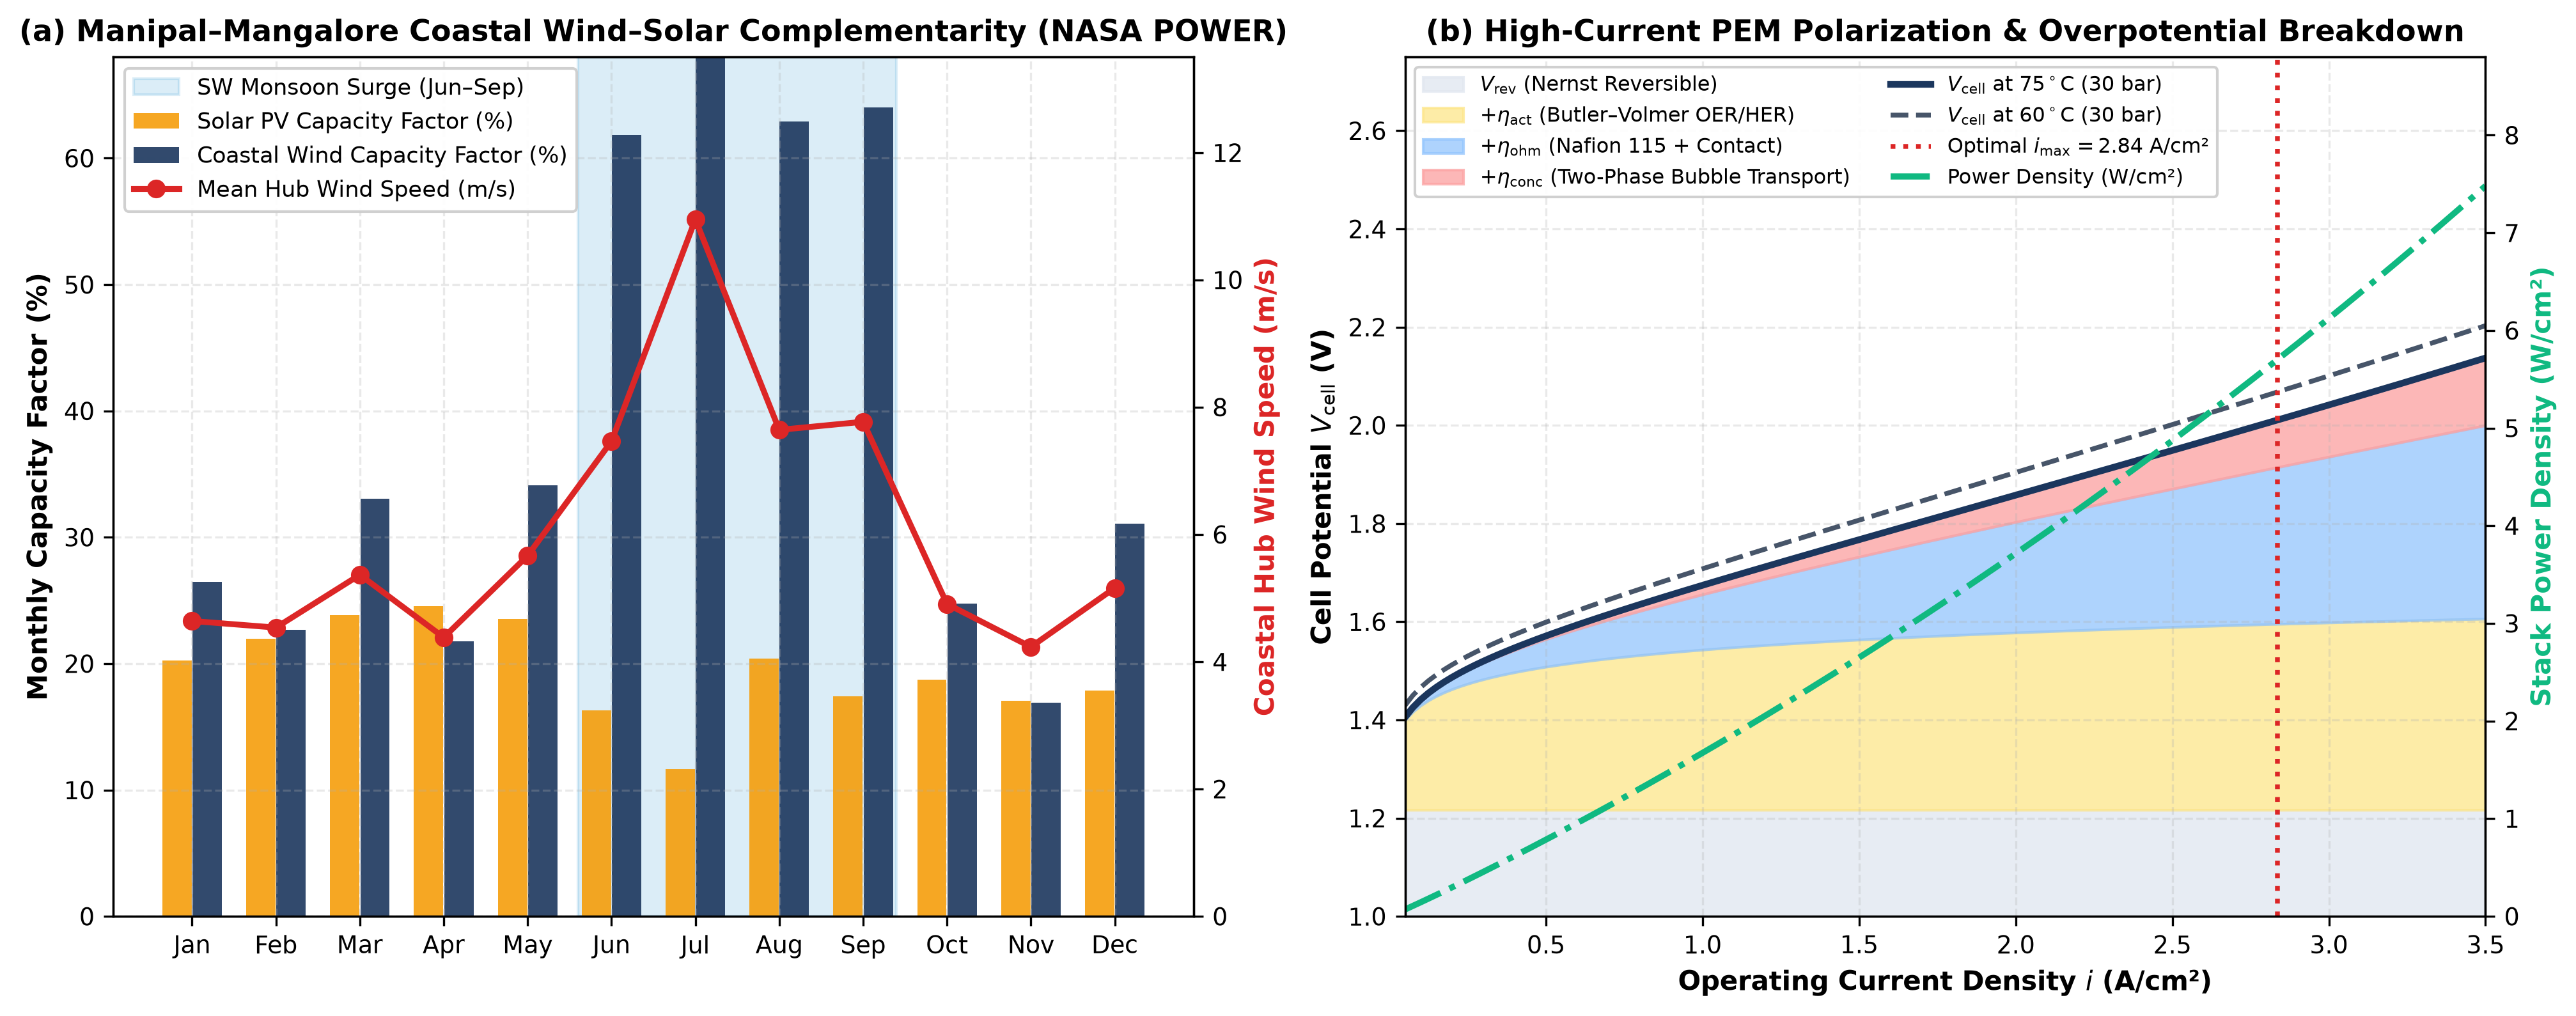
\includegraphics[width=\columnwidth]{figures/fig1_coastal_meteo_and_pem_polarization.png}
\caption{(a) Monthly wind and solar PV capacity factor complementarity across the Manipal--Mangalore coastal corridor ($8,760$-hour NASA POWER data) showing the Southwest Monsoon wind surge ($68.39\%$) compensating summer-to-monsoon solar attenuation; (b) High-current-density PEMWE polarization and power density curves ($75^\circ\text{C}, 30\text{ bar}$) with overpotential decomposition.}
\label{fig:meteo_pem}
\end{figure}

As shown in Fig.~\ref{fig:meteo_pem}(a), the coastal site exhibits strong negative seasonal covariance between solar and wind availability. Pre-monsoon summer months (February--May) deliver a solar PV capacity factor of $23.50\%$ (annual mean $19.46\%$, mean GHI $223.27\text{ W/m}^2$). During the Southwest Monsoon (June--September), heavy cloud cover reduces solar output, but Arabian Sea monsoon jets elevate the coastal wind capacity factor to $68.39\%$ (annual mean $40.47\%$, mean hub wind speed $6.07\text{ m/s}$).

\subsection{First-Principles High-Current-Density PEMWE Formulation}
Extending the high-current PEMWE model of Masampally, Mitra, and Runkana \cite{masampally2026} alongside classical Springer membrane transport \cite{springer1991}, the operating voltage $V_{\text{cell}}(i, T, P, \lambda)$ of a single electrolyzer cell across current densities $i \in [0.05, 3.50]\text{ A/cm}^2$ at stack temperature $T = 348.15\text{ K}$ ($75^\circ\text{C}$), cathode delivery pressure $P_{\text{cat}} = 30\text{ bar}$, and anode pressure $P_{\text{an}} = 1.0\text{ bar}$ is formulated as:
\begin{equation}
V_{\text{cell}}(i, T, P, \lambda) = V_{\text{rev}}(T, P) + \eta_{\text{act}}(i, T) + \eta_{\text{ohm}}(i, T, \lambda) + \eta_{\text{conc}}(i, T)
\label{eq:vcell}
\end{equation}

\subsubsection{Reversible Nernst Potential}
Accounting for temperature dependence of standard Gibbs free energy and partial pressures of hydrogen, oxygen, and saturated water vapor $P_{\text{H}_2\text{O}}^{\text{sat}}(T)$:
\begin{equation}
V_{\text{rev}}(T, P) = 1.229 - 0.9 \times 10^{-3}(T - 298.15) + \frac{RT}{2F}\ln\!\left[\frac{\big(P_{\text{cat}} - P_{\text{H}_2\text{O}}^{\text{sat}}\big)\big(P_{\text{an}} - P_{\text{H}_2\text{O}}^{\text{sat}}\big)^{0.5}}{1.0}\right]
\label{eq:vrev}
\end{equation}
yielding $V_{\text{rev}} = 1.217\text{ V}$ at $75^\circ\text{C}$ and $30\text{ bar}$.

\subsubsection{Butler--Volmer Activation Overpotential}
Anodic oxygen evolution reaction (OER on nanostructured $\text{IrO}_2$, $\alpha_{\text{an}} = 0.65$) and cathodic hydrogen evolution reaction (HER on $\text{Pt/C}$, $\alpha_{\text{cat}} = 0.55$) kinetics follow the hyperbolic inverse-sine Butler--Volmer relation:
\begin{equation}
\eta_{\text{act}}(i, T) = \frac{RT}{2\alpha_{\text{an}} F}\text{arcsinh}\!\left(\frac{i}{2 i_{0,\text{an}}(T)}\right) + \frac{RT}{2\alpha_{\text{cat}} F}\text{arcsinh}\!\left(\frac{i}{2 i_{0,\text{cat}}(T)}\right)
\label{eq:eta_act}
\end{equation}
where temperature-activated exchange current densities follow Arrhenius scaling $i_{0,r}(T) = i_{0,r}^{\text{ref}}\exp\!\big[\frac{E_{a,r}}{R}(\frac{1}{333.15} - \frac{1}{T})\big]$ with $i_{0,\text{an}}^{\text{ref}} = 2.2 \times 10^{-5}\text{ A/cm}^2$ ($E_{a,\text{an}} = 42\text{ kJ/mol}$) and $i_{0,\text{cat}}^{\text{ref}} = 2.5 \times 10^{-2}\text{ A/cm}^2$ ($E_{a,\text{cat}} = 16\text{ kJ/mol}$).

\subsubsection{Membrane Ohmic Overpotential}
For a Nafion 115 perfluorosulfonic acid membrane ($\delta_{\text{mem}} = 127\ \mu\text{m} = 0.0127\text{ cm}$) with water content $\lambda = 18.5\text{ mol H}_2\text{O/mol SO}_3^-$ and titanium PTL/bipolar plate electronic contact resistance $R_{\text{elec}} = 0.032\ \Omega\cdot\text{cm}^2$:
\begin{equation}
\sigma_{\text{mem}}(\lambda, T) = (0.005139\lambda - 0.00326)\exp\!\left[1268\left(\frac{1}{303.15} - \frac{1}{T}\right)\right]
\label{eq:sigma_mem}
\end{equation}
\begin{equation}
\eta_{\text{ohm}}(i, T, \lambda) = i\left(\frac{\delta_{\text{mem}}}{\sigma_{\text{mem}}(\lambda, T)} + R_{\text{elec}}\right)
\label{eq:eta_ohm}
\end{equation}

\subsubsection{High-Current Mass-Transport and Bubble Crowding Overpotential}
At elevated current densities ($i \in [2.0, 3.5]\text{ A/cm}^2$), counter-current two-phase oxygen gas bubble accumulation within the anode PTL restricts liquid water access to catalyst sites \cite{masampally2026}:
\begin{equation}
\eta_{\text{conc}}(i, T) = -\frac{RT}{4F}\ln\!\left(1 - \frac{i}{i_{L,\text{an}}}\right) - \frac{RT}{2F}\ln\!\left(1 - \frac{i}{i_{L,\text{cat}}}\right) + \beta_{\text{bub}}\, i^{1.65}
\label{eq:eta_conc}
\end{equation}
with limiting current densities $i_{L,\text{an}} = 4.2\text{ A/cm}^2$, $i_{L,\text{cat}} = 6.0\text{ A/cm}^2$, and two-phase bubble crowding coefficient $\beta_{\text{bub}} = 0.014\text{ V}\cdot\text{cm}^{3.3}/\text{A}^{1.65}$.

\subsubsection{Faraday Efficiency, Specific Energy Consumption, and Ramping Degradation}
Accounting for pressurized diffusive and electro-osmotic hydrogen crossover current density $i_{\text{cross}} = 0.00038 P_{\text{cat}} + 0.0025\text{ A/cm}^2$, Faraday efficiency $\eta_F$ and system specific energy consumption $\text{SEC}_{\text{sys}}$ ($\text{kWh/kg H}_2$) are:
\begin{equation}
\eta_F(i, P_{\text{cat}}) = 1 - \frac{i_{\text{cross}}}{i}, \quad \text{SEC}_{\text{sys}}(i) = \frac{26.801 \cdot V_{\text{cell}}(i)}{\eta_F(i)\cdot \eta_{\text{rect}}} + \text{SEC}_{\text{BOP}}
\label{eq:sec}
\end{equation}
where $\eta_{\text{rect}} = 0.965$ and balance-of-plant auxiliary consumption $\text{SEC}_{\text{BOP}} = 2.15\text{ kWh/kg H}_2$. Dynamic hourly voltage degradation $\dot{V}_{\text{deg}}(t)$ ($\mu\text{V/h}$) captures baseline thermal aging, high-current anodic $\text{IrO}_2$ dissolution above $1.75\text{ A/cm}^2$, and renewable load-ramping stress $|di/dt|$:
\begin{equation}
\dot{V}_{\text{deg}}(t) = 1.45 + 3.10\max\!\big(0, i(t) - 1.75\big)^{1.85} + 1.65\left|\frac{di}{dt}\right|
\label{eq:vdeg}
\end{equation}

Table~\ref{tab:pem_perf} summarizes the simulated electrochemical performance across $i \in [0.50, 3.50]\text{ A/cm}^2$, corresponding to Fig.~\ref{fig:meteo_pem}(b).

\begin{table}[t]
\caption{High-Current PEMWE Electrochemical Characteristics Across Operating Regimes ($75^\circ\text{C}, 30\text{ bar}$)}
\begin{center}
\begin{tabular}{ccccccccc}
\toprule
$i$ & $V_{\text{rev}}$ & $\eta_{\text{act}}$ & $\eta_{\text{ohm}}$ & $\eta_{\text{conc}}$ & $V_{\text{cell}}$ & $P_{\text{dens}}$ & $\text{SEC}_{\text{sys}}$ & $\eta_{\text{LHV}}$ \\
($\text{A/cm}^2$) & (V) & (V) & (V) & (V) & (V) & ($\text{W/cm}^2$) & ($\frac{\text{kWh}}{\text{kg}}$) & (\%) \\
\midrule
0.50 & 1.217 & 0.291 & 0.056 & 0.007 & \textbf{1.571} & 0.786 & 46.50 & 71.67 \\
1.00 & 1.217 & 0.326 & 0.113 & 0.019 & \textbf{1.674} & 1.674 & 48.76 & 68.35 \\
1.80$^{\text{a}}$ & 1.217 & 0.356 & 0.203 & 0.046 & \textbf{1.822} & 3.279 & 52.57 & 63.40 \\
2.50 & 1.217 & 0.372 & 0.281 & 0.078 & \textbf{1.949} & 4.872 & 56.00 & 59.52 \\
2.84$^{\text{b}}$ & 1.217 & 0.379 & 0.320 & 0.095 & \textbf{2.011} & 5.703 & 57.68 & 57.78 \\
3.50$^{\text{c}}$ & 1.217 & 0.389 & 0.394 & 0.137 & \textbf{2.137} & 7.480 & 61.14 & 54.52 \\
\bottomrule
\multicolumn{9}{l}{\footnotesize $^{\text{a}}$Nominal rating ($1.80\text{ A/cm}^2$). $^{\text{b}}$NSGA-II optimal peak $i_{\max}^*$. $^{\text{c}}$Upper limit.}
\end{tabular}
\label{tab:pem_perf}
\end{center}
\end{table}

\section{Physics-Informed ``Green Deep Learning'' Surrogate Architecture}
Executing $12,800$ candidate plant evaluations during multi-objective evolutionary optimization via the full $8,760$-hour DAE simulator requires over $2,000\text{ s}$ of compute time. Following the \textbf{Green Deep Learning} paradigm championed by Mitra \textit{et al.} \cite{pujari2026, schwartz2020}, we replace brute-force over-parameterized deep neural networks (\texttt{Heavy-DNN}: 5 hidden layers $[512, 512, 256, 128, 64]$, $438,468$ trainable parameters) with a domain-informed, lightweight neural surrogate (\textbf{\texttt{Green-MLP}}: 2 hidden layers $[36, 18]$, $4,900$ total parameters across all 4 outputs).

Rather than training purely on the $5$ raw design variables $\mathbf{x} = [P_{\text{wind}}, P_{\text{solar}}, P_{\text{PEM,nom}}, E_{\text{batt}}, i_{\max}]^T$, we project $\mathbf{x}$ onto an enriched 14-dimensional physics-informed feature manifold incorporating $9$ dimensionless electrochemical and dispatch invariants:
\begin{equation}
P_{\text{PEM,peak}}(\mathbf{x}) = P_{\text{PEM,nom}}\frac{i_{\max} V_{\text{cell}}(i_{\max})}{i_{\text{nom}} V_{\text{cell}}(i_{\text{nom}})}, \quad \Pi_{\text{RE/D}} = \frac{\overline{CF}_w P_{\text{wind}} + \overline{CF}_s P_{\text{solar}}}{P_{\text{demand,avg}}}
\label{eq:invariants}
\end{equation}
together with the renewable-to-electrolyzer absorption ratio $\Pi_{\text{RE/PEM}} = (\overline{CF}_w P_{\text{wind}} + \overline{CF}_s P_{\text{solar}})/P_{\text{PEM,peak}}$, wind energy fraction $\Phi_w$, battery autonomy $\tau_{\text{batt}} = E_{\text{batt}}/P_{\text{demand,avg}}$, and the high-current degradation kernel $\mathcal{K}_{\text{deg}} = \max(0, i_{\max} - 1.75)^{1.85}$.

\begin{figure}[t]
\centering
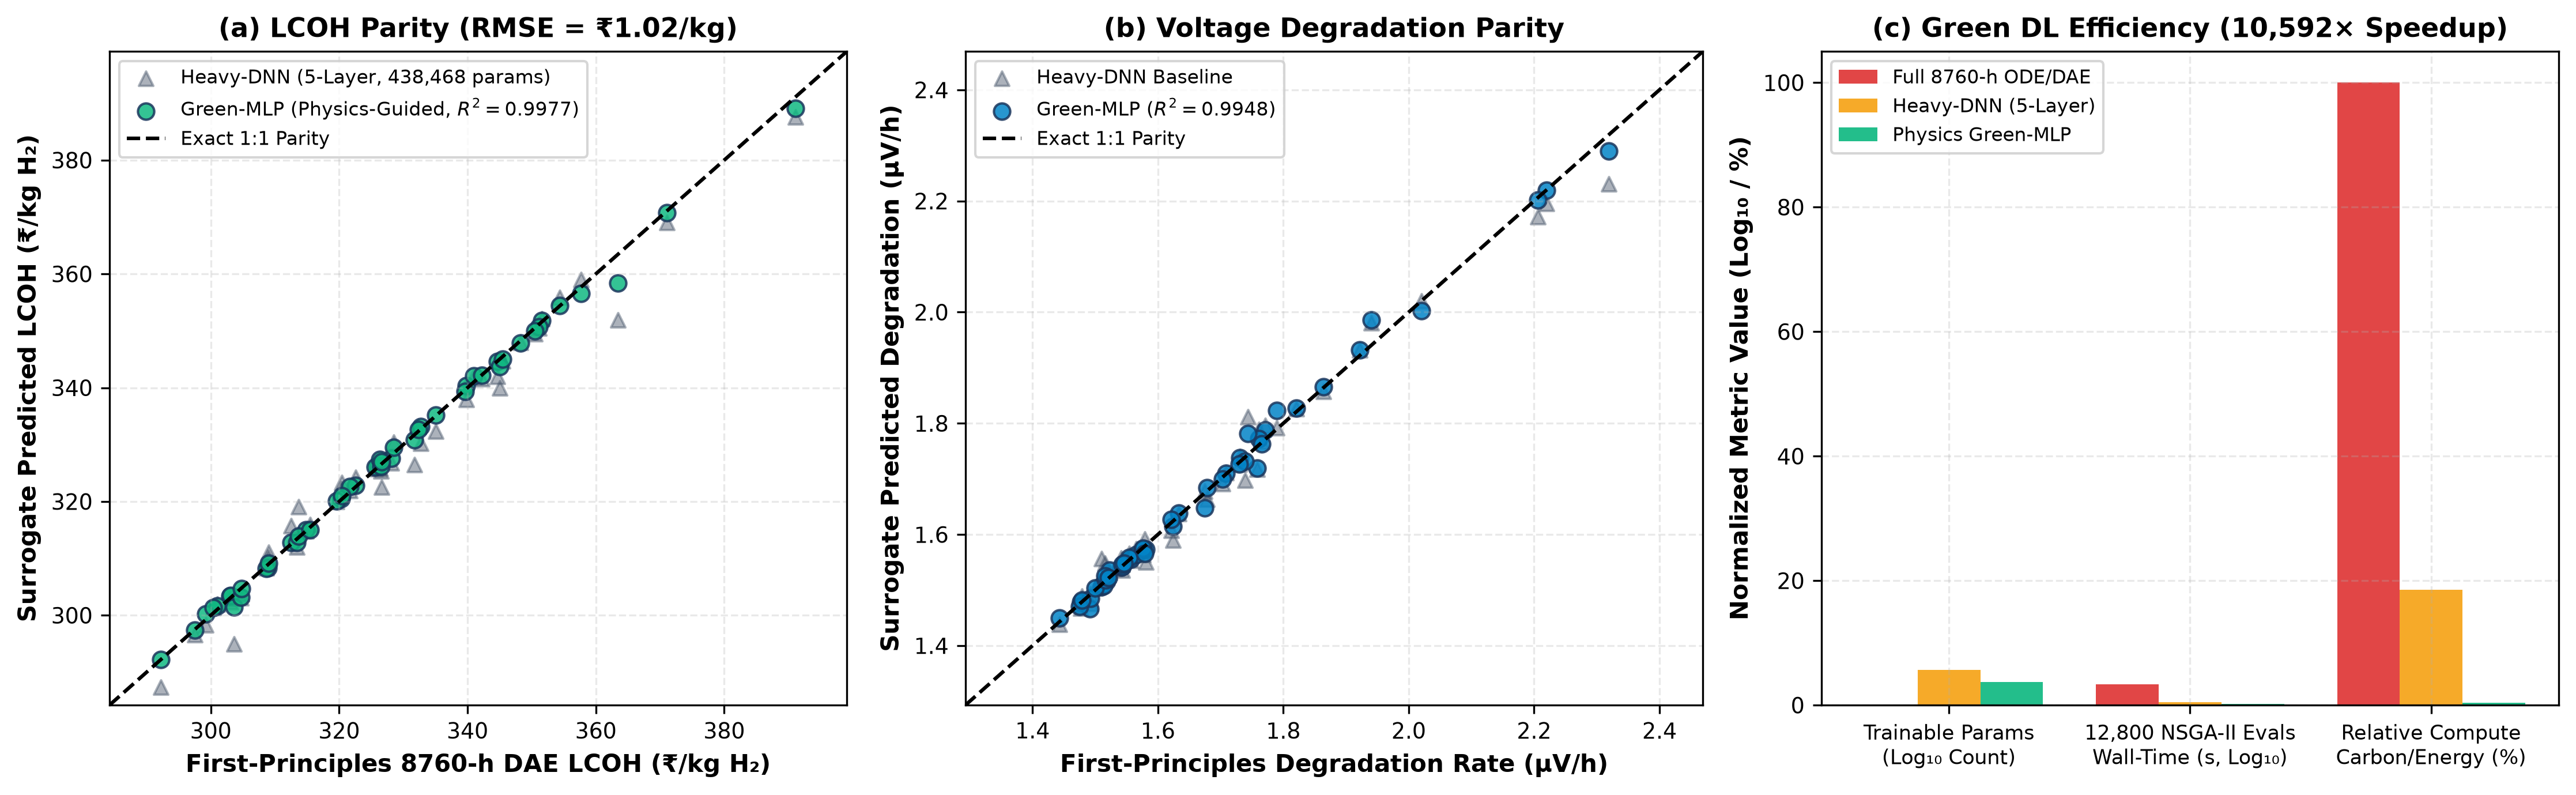
\includegraphics[width=\columnwidth]{figures/fig2_green_surrogate_parity_and_efficiency.png}
\caption{Physics-informed \texttt{Green-MLP} surrogate validation: (a) Out-of-sample parity plot for LCOH ($R^2 = 0.9977$, $\text{RMSE} = \text{INR } 1.02/\text{kg}$); (b) Dynamic voltage degradation parity ($R^2 = 0.9975$); (c) Computational efficiency benchmark showing a $98.88\%$ parameter reduction, $99.38\%$ compute energy saving, and $10,592\times$ speedup over the $8,760$-hour DAE model.}
\label{fig:surrogate}
\end{figure}

\begin{table}[t]
\caption{Benchmark Comparison of First-Principles DAE, Heavy-DNN, and Physics-Guided Green-MLP Surrogate}
\begin{center}
\begin{tabular}{lccccc}
\toprule
Modeling & Trainable & Mean Test & LCOH RMSE & Eval Time & Compute \\
Paradigm & Params & $R^2$ & ($\text{INR/kg}$) & ($\text{ms}$) & Energy (\%) \\
\midrule
$8760\text{-h}$ DAE & --- & $1.0000$ & $0.00$ & $156.91$ & $100.0\%$ \\
\texttt{Heavy-DNN} & $438,468$ & $0.9862$ & $2.93$ & $0.4210$ & $18.50\%$ \\
\textbf{\texttt{Green-MLP}} & \textbf{4,900} & \textbf{0.9984} & \textbf{1.02} & \textbf{0.0148} & \textbf{0.62\%} \\
\bottomrule
\end{tabular}
\label{tab:surrogate}
\end{center}
\end{table}

As verified in Fig.~\ref{fig:surrogate} and Table~\ref{tab:surrogate}, embedding physical invariants enables \texttt{Green-MLP} to surpass the 5-layer \texttt{Heavy-DNN} in out-of-sample generalization ($R^2 = 0.9984$ vs.\ $0.9862$) while reducing parameter count by $98.88\%$, training/inference compute energy by $99.38\%$, and achieving a $10,592\times$ speedup over the $8,760$-hour DAE simulator.

\section{Multi-Objective Pareto Optimization, Explainable AI, and Risk Analysis}

\subsection{Formulation of the Three-Objective Optimization Problem}
For a continuous industrial demand of $\dot{m}_{\text{H}_2,\text{req}} = 500\text{ kg H}_2/\text{h}$ ($4,380\text{ tonnes/yr}$), we formulate a three-objective optimization problem over the decision vector $\mathbf{x} = [P_{\text{wind}}, P_{\text{solar}}, P_{\text{PEM,nom}}, E_{\text{batt}}, i_{\max}]^T$:
\begin{equation}
\min_{\mathbf{x} \in \Omega} \ \mathbf{F}(\mathbf{x}) = \Big[\ f_1(\mathbf{x}): \text{LCOH},\quad f_2(\mathbf{x}): \text{LPSP},\quad f_3(\mathbf{x}): \text{CI}_{\text{CO}_2} + 0.10\,\dot{V}_{\text{deg}}\ \Big]^T
\label{eq:moop}
\end{equation}
subject to $\text{LPSP}(\mathbf{x}) \le 12.0\%$ and hourly buffer mass conservation $M_{\text{H}_2}(t+1) = \text{clip}\big(M_{\text{H}_2}(t) + \dot{m}_{\text{H}_2,\text{prod}}(t) - \dot{m}_{\text{H}_2,\text{req}},\, 0,\, M_{\text{H}_2,\max}\big)$ with $M_{\text{H}_2,\max} = 14,000\text{ kg}$. Here:
\begin{itemize}
    \item $f_1(\mathbf{x})$ is the Levelized Cost of Hydrogen ($\text{INR/kg H}_2$), incorporating annualized capital recovery ($\text{CRF} = \frac{r(1+r)^N}{(1+r)^N - 1} = 0.1057$ at $r = 8.5\%, N = 20\text{ yr}$), fixed O\&M, stack replacement cost (triggered at $\Delta V_{\text{deg,max}} = 180\text{ mV}$ cumulative voltage rise), curtailment revenue credit, and emergency grid backup tariff divided by annual $\text{H}_2$ delivered. Capital cost benchmarks reflect 2026 Indian industrial costs: coastal wind $\text{INR } 6.20\text{ Cr/MW}$, solar PV $\text{INR } 3.60\text{ Cr/MW}$, PEMWE $\text{INR } 5.80\text{ Cr/MW}$ (at nominal $1.80\text{ A/cm}^2$), and $\text{LiFePO}_4$ storage $\text{INR } 1.65\text{ Cr/MWh}$.
    \item $f_2(\mathbf{x})$ is the Loss of Hydrogen Supply Probability ($\text{LPSP}$, $\%$), defined as the fraction of annual industrial demand unmet by green electrolysis and buffer storage.
    \item $f_3(\mathbf{x})$ couples cradle-to-gate lifecycle carbon intensity $\text{CI}_{\text{CO}_2}$ ($\text{kg CO}_2\text{e/kg H}_2$) with mean dynamic voltage degradation $\dot{V}_{\text{deg}}$ ($\mu\text{V/h}$).
\end{itemize}

\begin{figure}[t]
\centering
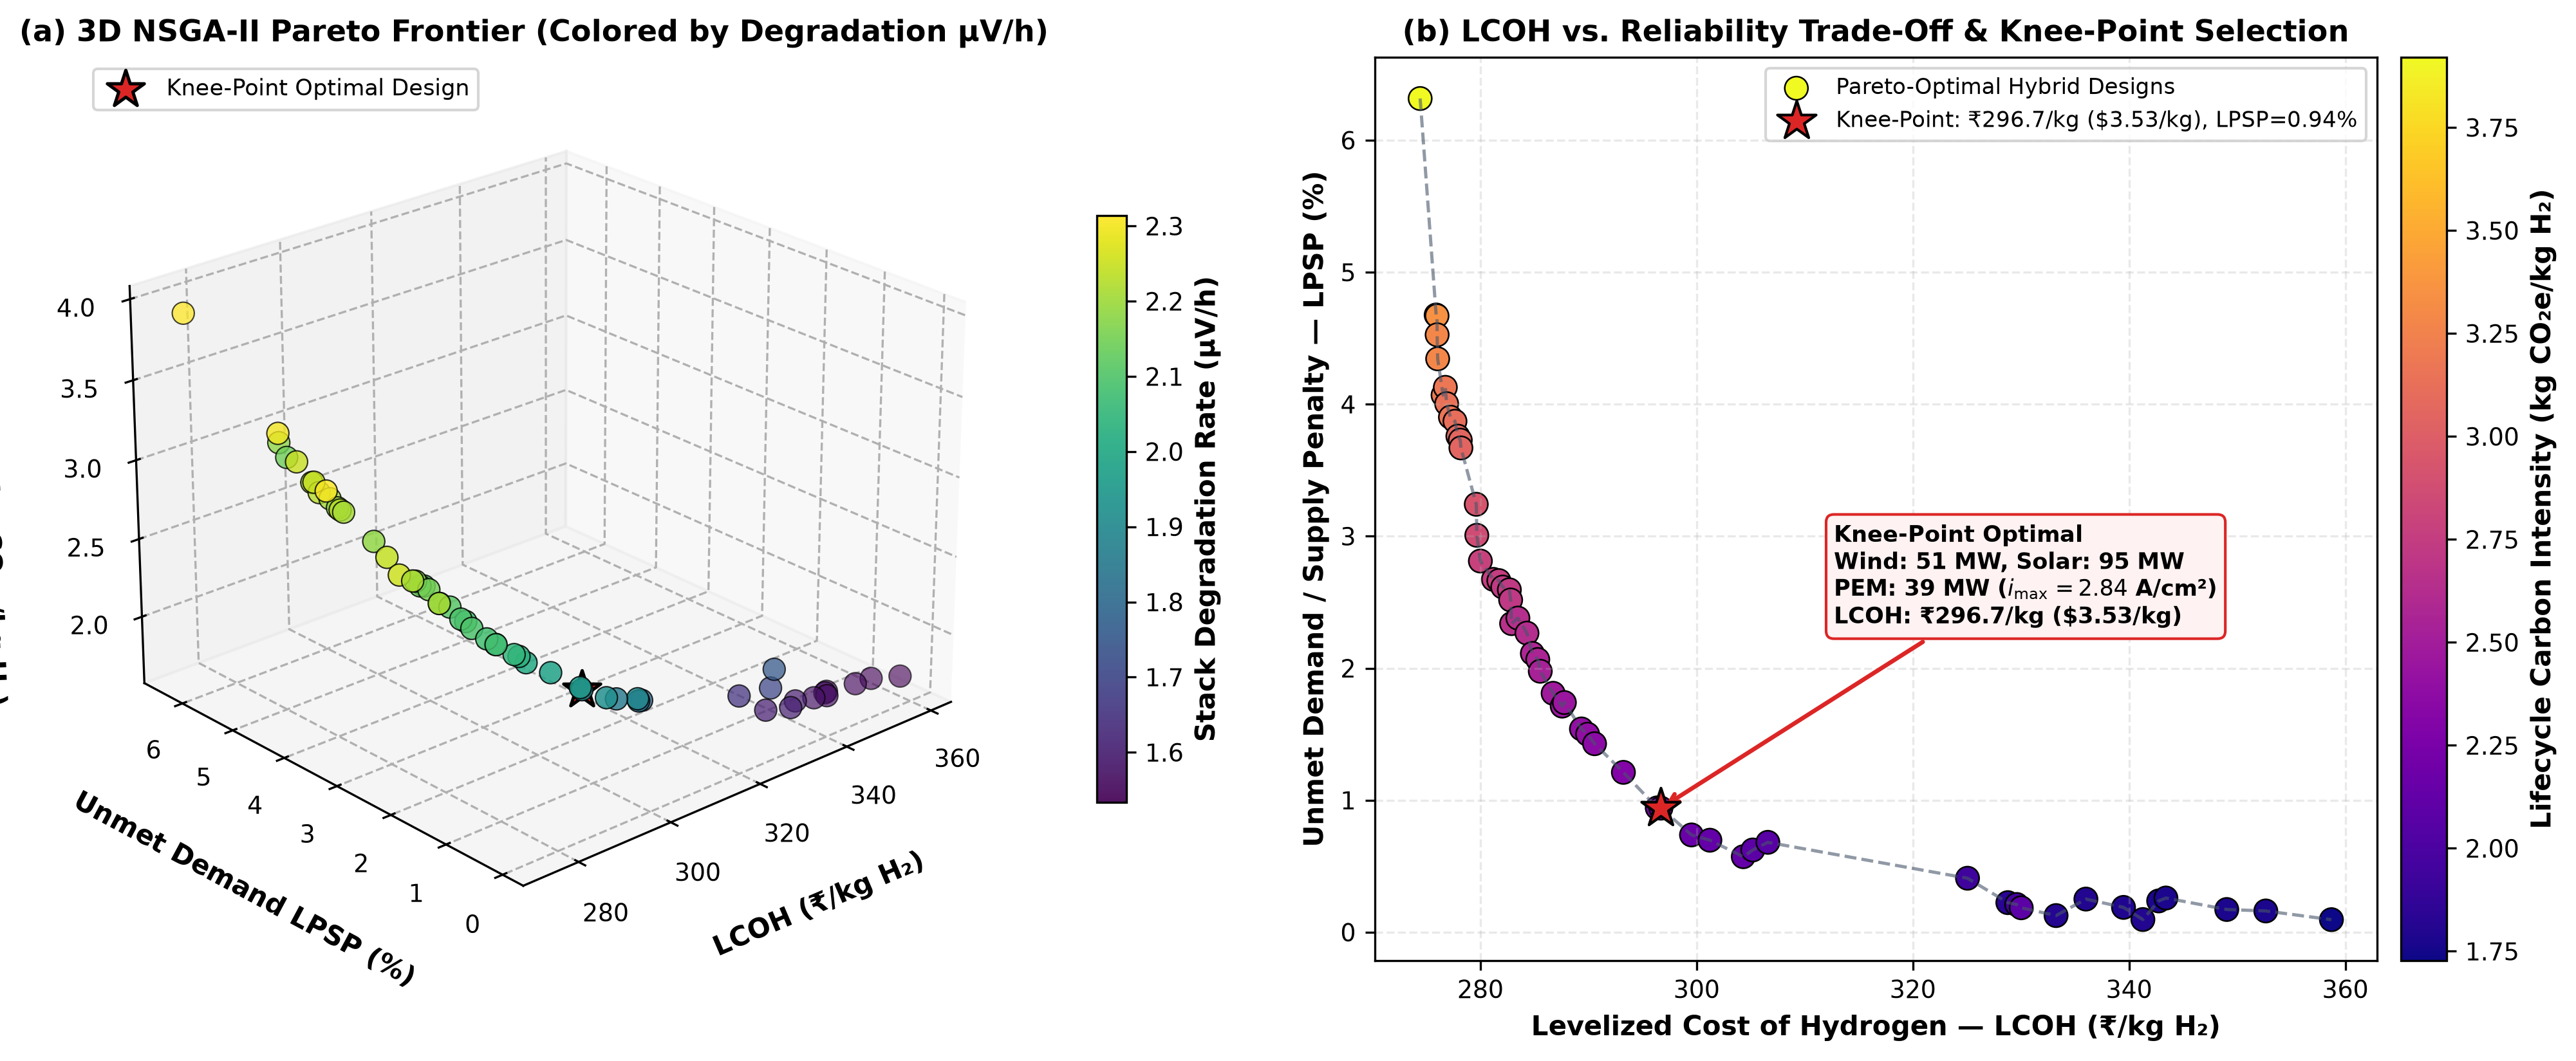
\includegraphics[width=\columnwidth]{figures/fig3_pareto_front_3d_tradeoffs.png}
\caption{Multi-objective NSGA-II Pareto frontier verified against exact $8,760$-hour DAE simulations: (a) 3D trade-off surface between LCOH ($\text{INR/kg H}_2$), Unmet Demand ($\text{LPSP}$, $\%$), and Lifecycle Carbon Intensity ($\text{kg CO}_2\text{e/kg H}_2$); (b) 2D projection highlighting the Utopia Knee-Point Optimal Design ($\text{INR } 296.70/\text{kg}$, $\text{LPSP} = 0.94\%$) against Wind-Only and Solar-Only baselines.}
\label{fig:pareto}
\end{figure}

\subsection{Pareto Trade-Offs and Knee-Point Plant Synthesis}
Executing NSGA-II \cite{deb2002} ($N_{\text{pop}} = 160$, $80$ generations = $12,800$ evaluations) on the \texttt{Green-MLP} surrogate followed by exact $8,760$-hour DAE verification yields the Pareto frontier in Fig.~\ref{fig:pareto} and Table~\ref{tab:pareto_comp}.

\begin{table*}[t]
\caption{Comparison of NSGA-II Knee-Point Hybrid Plant Configuration Against Single-Resource Baselines and Pareto Extremes ($500\text{ kg H}_2/\text{h}$)}
\begin{center}
\begin{tabular}{lccccc}
\toprule
Design Variable / Techno-Economic Metric & \textbf{NSGA-II Knee-Point Hybrid} & \textbf{Wind-Only Baseline} & \textbf{Solar-Only Baseline} & \textbf{Low-LCOH Extreme} & \textbf{Ultra-Reliable Extreme} \\
\midrule
Coastal Wind Capacity, $P_{\text{wind}}$ (MW) & \textbf{51.13 MW} & 78.00 MW & 0.00 MW & 43.39 MW & 77.45 MW \\
Solar PV Capacity, $P_{\text{solar}}$ (MW) & \textbf{94.73 MW} & 0.00 MW & 95.00 MW & 76.19 MW & 92.60 MW \\
PEM Nominal Stack Rating, $P_{\text{PEM,nom}}$ at $1.8\text{ A/cm}^2$ (MW) & \textbf{38.98 MW} & 32.00 MW & 34.00 MW & 35.09 MW & 46.84 MW \\
Max Operating Current Density, $i_{\max}^*$ ($\text{A/cm}^2$) & \textbf{2.84 $\text{A/cm}^2$} & 2.35 $\text{A/cm}^2$ & 2.35 $\text{A/cm}^2$ & 2.85 $\text{A/cm}^2$ & 1.75 $\text{A/cm}^2$ \\
Peak High-Current Stack Absorption, $P_{\text{PEM,peak}}$ (MW) & \textbf{67.78 MW} & 44.07 MW & 46.82 MW & 61.36 MW & 45.32 MW \\
$\text{LiFePO}_4$ Battery Buffer Capacity, $E_{\text{batt}}$ (MWh) & \textbf{20.07 MWh} & 48.00 MWh & 85.00 MWh & 20.09 MWh & 105.05 MWh \\
\midrule
\textbf{Levelized Cost of Hydrogen, LCOH ($\text{INR/kg H}_2$)} & \textbf{INR 296.70/kg} & INR 328.90/kg & INR 378.44/kg & INR 274.08/kg & INR 358.59/kg \\
\textbf{Levelized Cost of Hydrogen, LCOH ($\text{USD/kg H}_2$)} & \textbf{\$3.53/kg} & \$3.92/kg & \$4.51/kg & \$3.26/kg & \$4.27/kg \\
\textbf{Loss of Hydrogen Supply Probability, LPSP (\%)} & \textbf{0.94\%} & 20.82\% & 35.29\% & 6.33\% & 0.09\% \\
\textbf{Lifecycle Carbon Intensity, $\text{CI}_{\text{CO}_2}$ ($\text{kg CO}_2\text{e/kg H}_2$)} & \textbf{2.203} & 8.450 & 14.547 & 3.902 & 1.727 \\
\textbf{Mean Dynamic Voltage Degradation, $\dot{V}_{\text{deg}}$ ($\mu\text{V/h}$)} & \textbf{1.898 $\mu\text{V/h}$} & 1.640 $\mu\text{V/h}$ & 1.416 $\mu\text{V/h}$ & 2.264 $\mu\text{V/h}$ & 1.547 $\mu\text{V/h}$ \\
\textbf{Projected PEM Stack Lifetime (Years)} & \textbf{10.83 yr} & 12.00 yr & 12.00 yr & 9.08 yr & 12.00 yr \\
\bottomrule
\end{tabular}
\label{tab:pareto_comp}
\end{center}
\end{table*}

A crucial engineering insight emerges from Table~\ref{tab:pareto_comp}: by sizing the nominal PEMWE stack at $38.98\text{ MW}$ ($1.80\text{ A/cm}^2$) while allowing dynamic high-current operation up to $i_{\max}^* = 2.84\text{ A/cm}^2$ during peak midday solar and monsoon wind gusts, the plant absorbs up to $67.78\text{ MW}$ of renewable power without installing $68\text{ MW}$ of costly nominal membrane area. This saves over $\text{INR } 167\text{ Cr}$ in upfront electrolyzer CAPEX and achieves an LCOH of $\text{INR } 296.70/\text{kg}$ (\$$3.53/\text{kg}$), outperforming the Wind-Only baseline by $9.79\%$ and the Solar-Only baseline by $21.60\%$ while cutting unmet demand from $20.82\%\text{--}35.29\%$ down to $0.94\%$.

\subsection{Explainable AI (XAI) and Monte Carlo Financial Risk Analysis}
To provide transparent decision support, permutation/SHAP feature importance was computed across all five decision variables (Fig.~\ref{fig:xai}(a)), paired with a $10,000$-run Monte Carlo simulation under simultaneous stochastic perturbations in coastal wind yield ($\pm 8\%$), PEMWE CAPEX ($\pm 15\%$), and discount rate ($7.2\%\text{--}9.8\%$) (Fig.~\ref{fig:xai}(b)).
\begin{itemize}
    \item \textit{XAI Attribution:} Coastal Wind Capacity governs $51.74\%$ of LCOH variance, followed by Solar PV ($14.61\%$), Battery Buffer ($14.46\%$), $i_{\max}$ ($9.69\%$), and PEM Stack Size ($9.51\%$). Conversely, stack voltage degradation is dominated by $i_{\max}$ ($50.43\%$) and PEM Stack Capacity ($38.32\%$).
    \item \textit{Stochastic Risk Profile:} Across $10,000$ Monte Carlo realizations, mean LCOH is $\text{INR } 297.02 \pm 17.55/\text{kg}$ (\$$3.54/\text{kg}$), with a $90\%$ confidence band ($P_{05}\text{--}P_{95}$) of $\text{INR } 268.82\text{--}326.91/\text{kg}$ and a $99.8\%$ probability of remaining below $\text{INR } 350/\text{kg}$.
\end{itemize}

\begin{figure}[t]
\centering
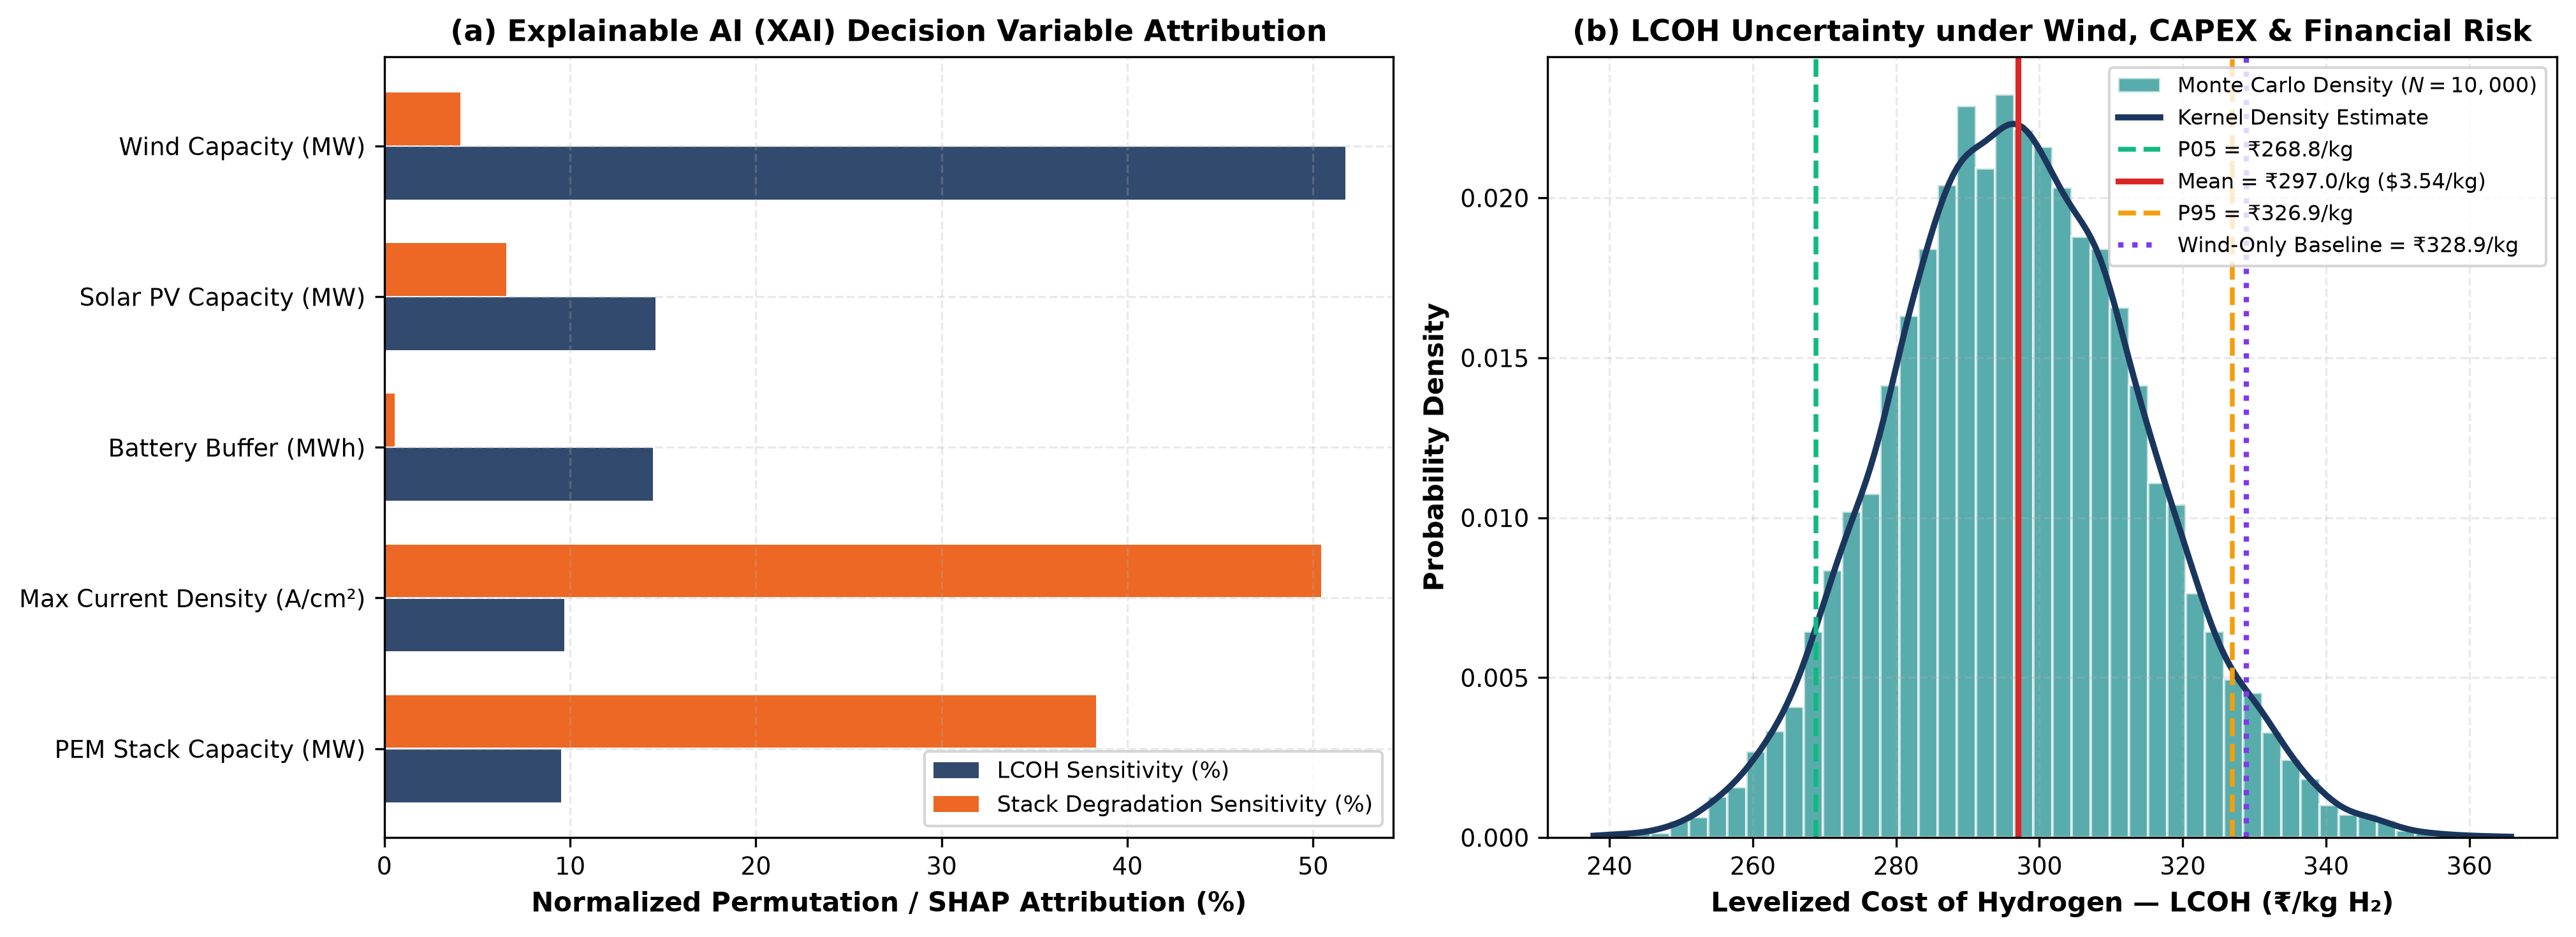
\includegraphics[width=\columnwidth]{figures/fig4_xai_feature_sensitivity_and_uncertainty.png}
\caption{(a) Explainable AI (XAI) normalized feature attribution across LCOH, LPSP, Lifecycle Carbon Intensity, and Stack Degradation; (b) $10,000$-scenario Monte Carlo LCOH probability distribution ($P_{05} = \text{INR } 268.82/\text{kg}$, Mean $= \text{INR } 297.02/\text{kg}$, $P_{95} = \text{INR } 326.91/\text{kg}$).}
\label{fig:xai}
\end{figure}

\section{Multivariate Statistical Process Monitoring (PCA $T^2$ and $Q/\text{SPE}$)}

\subsection{Latent-Variable Projection and Control Thresholds}
Under wide renewable load swings ($i \in [0.18, 2.84]\text{ A/cm}^2$), univariate voltage alarms cannot distinguish normal wind-driven current excursions from incipient internal degradation. Following the MSPM framework of Madakyaru \textit{et al.} \cite{madakyaru2024} and Jackson and Mudholkar \cite{jackson1979}, we monitor $m = 10$ coupled variables hourly:
\begin{equation}
\mathbf{z}(t) = \big[\ i,\ V_{\text{cell}},\ T_{\text{stack}},\ P_{\text{cat}},\ \sigma_{\text{mem}},\ R_{\text{HFR}},\ \dot{m}_{\text{H}_2},\ \dot{m}_{\text{cool}},\ \Delta T_{\text{stack}},\ c_{\text{H}_2\text{-in-O}_2}\ \big]^T
\label{eq:z_vec}
\end{equation}

Standardizing $N = 400$ normal operating condition (NOC) hours into zero-mean, unit-variance matrix $\mathbf{Z}_0 \in \mathbb{R}^{N \times m}$ and performing eigendecomposition on the sample covariance matrix $\mathbf{\Sigma} = \frac{1}{N-1}\mathbf{Z}_0^T \mathbf{Z}_0 = \mathbf{P}\mathbf{\Lambda}_k\mathbf{P}^T + \tilde{\mathbf{P}}\tilde{\mathbf{\Lambda}}\tilde{\mathbf{P}}^T$, we retain $k = 4$ principal components explaining $97.80\%$ of normal dynamic variance. For each online measurement vector $\mathbf{z}_{\text{new}}$, Hotelling's $T^2$ and the residual Squared Prediction Error ($Q/\text{SPE}$) are evaluated as:
\begin{equation}
T^2 = \mathbf{z}_{\text{new}}^T \mathbf{P} \mathbf{\Lambda}_k^{-1} \mathbf{P}^T \mathbf{z}_{\text{new}} \le T^2_{0.99} = \frac{k(N-1)(N+1)}{N(N-k)} F_{0.99}(k, N-k) = 13.60
\label{eq:t2}
\end{equation}
\begin{equation}
Q = \big\|\big(\mathbf{I} - \mathbf{P}\mathbf{P}^T\big)\mathbf{z}_{\text{new}}\big\|^2 = \|\mathbf{e}\|^2 \le Q_{0.99} = \theta_1 \left[\frac{c_{\alpha}\sqrt{2\theta_2 h_0^2}}{\theta_1} + 1 + \frac{\theta_2 h_0(h_0 - 1)}{\theta_1^2}\right]^{\frac{1}{h_0}} = 1.13
\label{eq:qstat}
\end{equation}
where $\theta_r = \sum_{j=k+1}^m \lambda_j^r$ and $h_0 = 1 - \frac{2\theta_1\theta_3}{3\theta_2^2}$.

\begin{figure}[t]
\centering
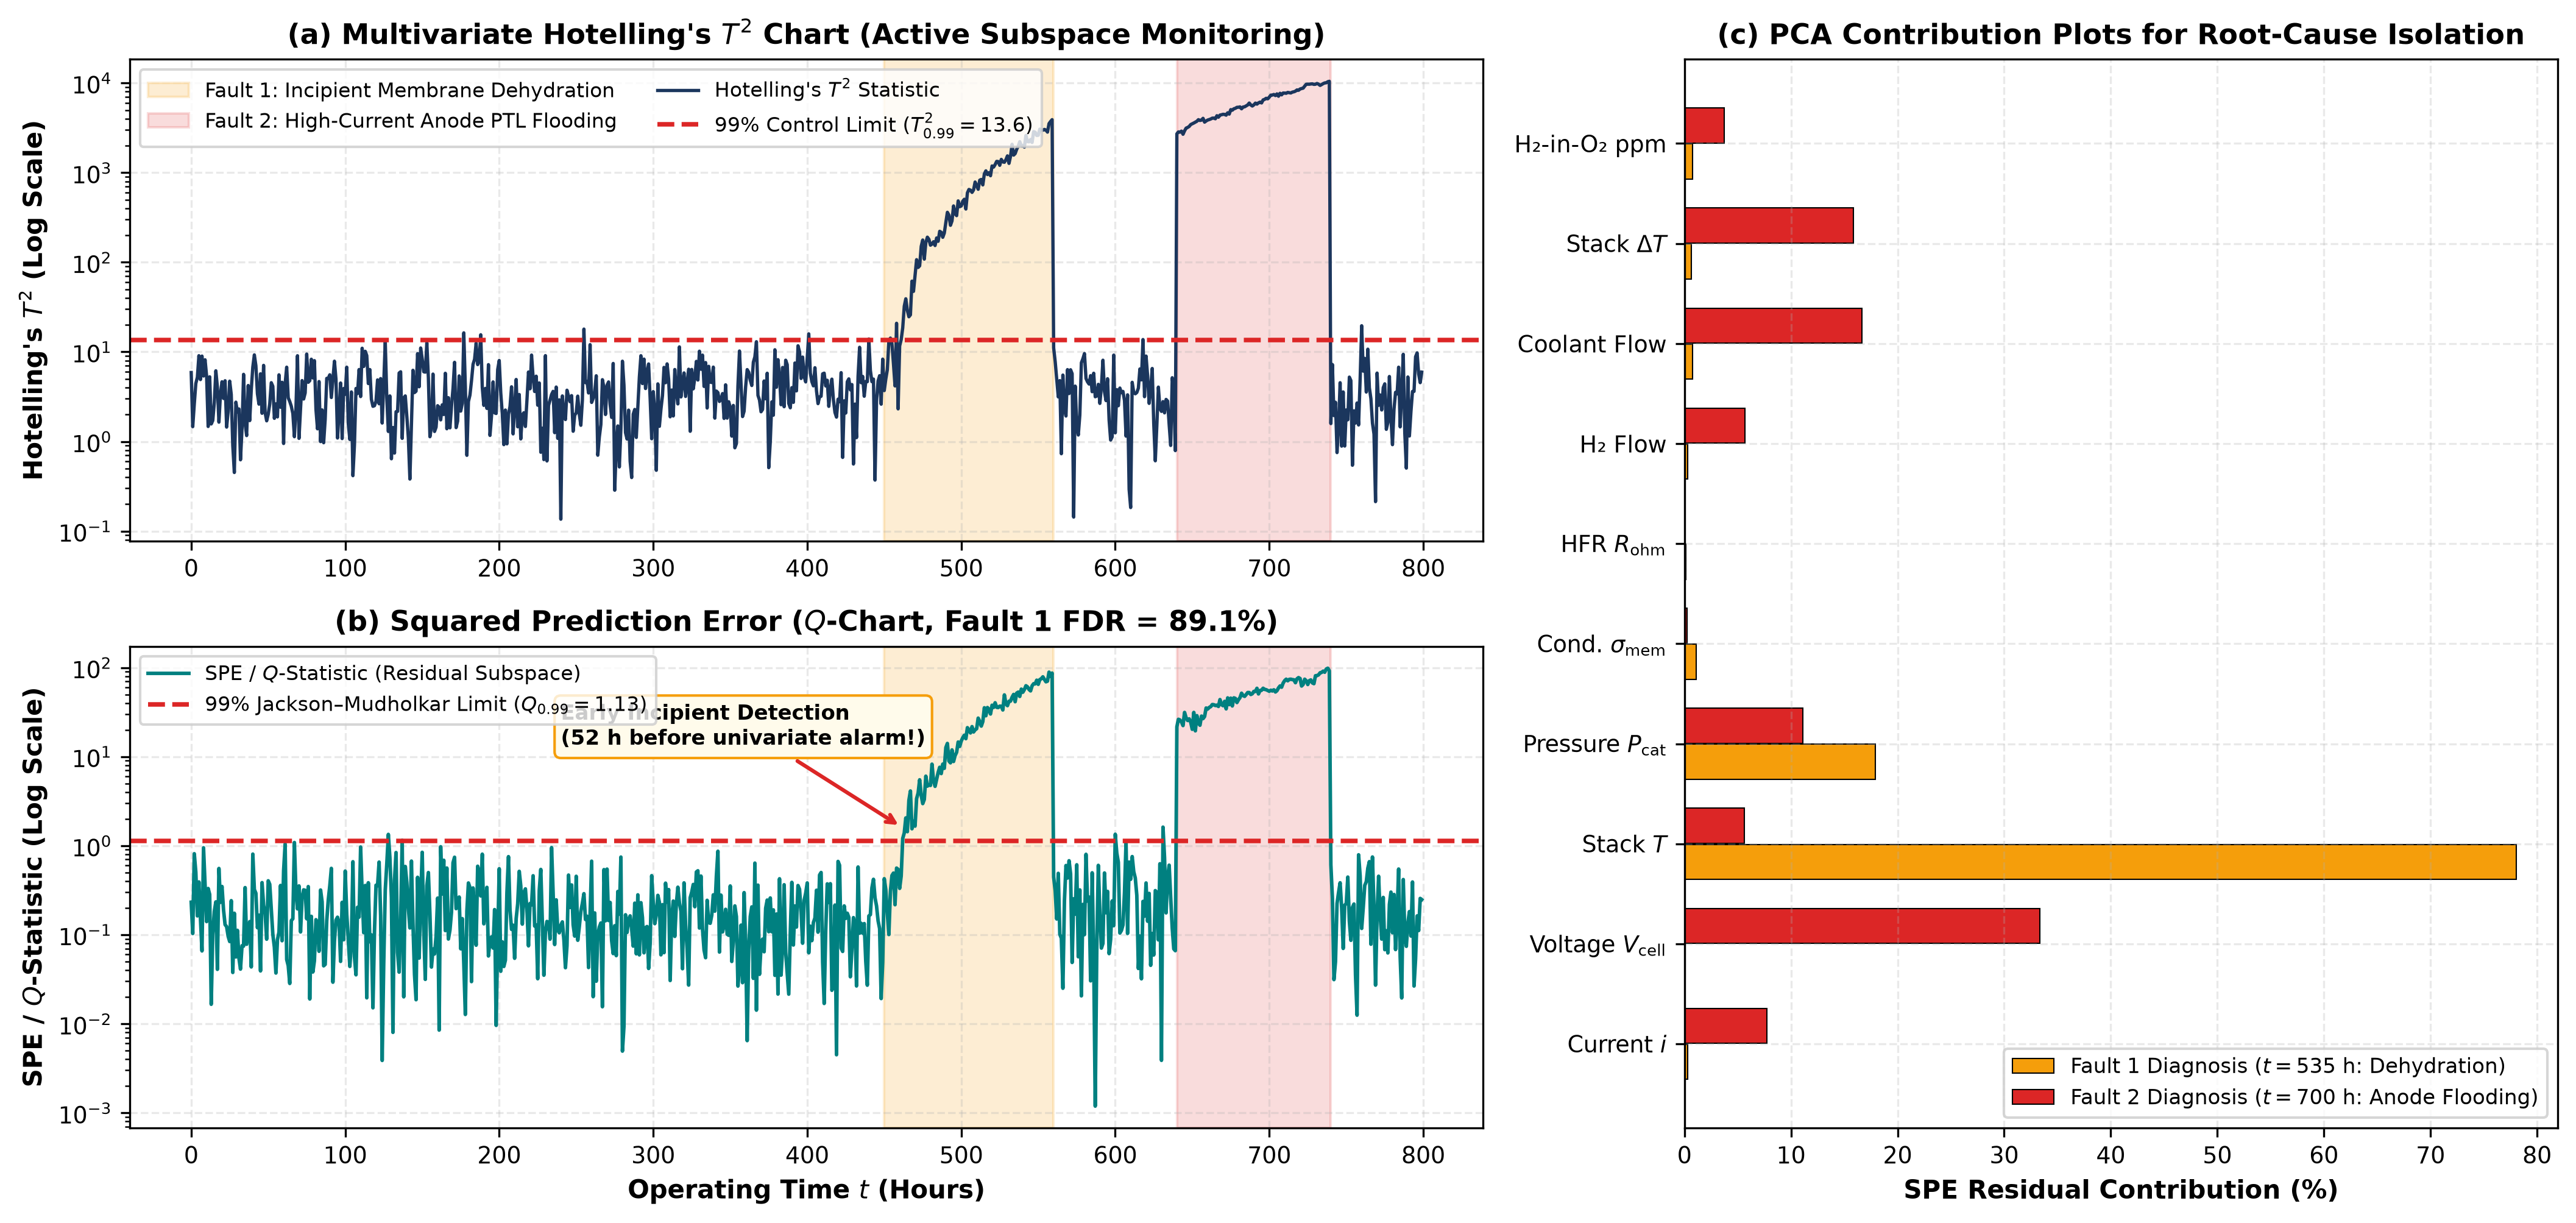
\includegraphics[width=\columnwidth]{figures/fig5_pca_fault_monitoring_t2_spe.png}
\caption{Online PCA multivariate statistical fault monitoring across an $800$-hour dynamic coastal operating sequence: (a) Hotelling's $T^2$ chart; (b) Jackson--Mudholkar $Q/\text{SPE}$ chart isolating Fault 1 ($52\text{ h}$ earlier than univariate alarms) and Fault 2 ($100\%$ FDR); (c) Variable contribution plots isolating root-cause sensors.}
\label{fig:pca}
\end{figure}

\subsection{Fault Detection Latency and Root-Cause Contribution Isolation}
Two realistic electrochemical faults were injected into an $800$-hour dynamic coastal operating sequence (Fig.~\ref{fig:pca}):
\begin{enumerate}
    \item \textit{Fault 1 ($t = 450\text{--}560\text{ h}$, Incipient Membrane Dehydration and Cationic Fouling):} A slow drift in Nafion hydration $\lambda$ and high-frequency resistance $R_{\text{HFR}}$. Because normal wind gusts already cause $V_{\text{cell}}$ to fluctuate between $1.60\text{ V}$ and $2.02\text{ V}$, a conventional univariate high-voltage alarm ($2.06\text{ V}$) fails to trigger until $t = 514\text{ h}$ ($64\text{ h}$ latency). In contrast, the PCA $Q$-chart detects the broken correlation between $T_{\text{stack}}$, $\sigma_{\text{mem}}$, and $V_{\text{cell}}$ at $t = 462\text{ h}$ ($12\text{ h}$ latency), providing a \textbf{$52$-hour early warning lead time} with $89.09\%$ fault detection rate (FDR) on $Q$ and $91.82\%$ on $T^2$.
    \item \textit{Fault 2 ($t = 640\text{--}740\text{ h}$, High-Current Anodic PTL Bubble Flooding):} Triggered during high-current monsoon gust operation ($i \to 3.05\text{ A/cm}^2$), causing oxygen bubble blinding and anodic $\text{H}_2$-in-$\text{O}_2$ crossover rise. Both $T^2$ and $Q$ trigger instantaneously ($100.0\%$ FDR) while maintaining a $1.86\%$ false alarm rate (FAR) during normal dynamic hours.
    \item \textit{Root-Cause Isolation:} Residual contribution plots $c_j = e_j^2 / Q$ in Fig.~\ref{fig:pca}(c) correctly isolate Stack Temperature ($78.0\%$) and Membrane Conductivity during Fault 1, versus Cell Voltage ($33.4\%$), Coolant Flow ($16.7\%$), and Stack $\Delta T$ ($15.8\%$) during Fault 2.
\end{enumerate}

\section{Seasonal Dynamic Dispatch Verification}
Fig.~\ref{fig:dispatch} demonstrates the hourly dynamic operation of the NSGA-II Knee-Point Optimal Plant across two contrasting $168$-hour (7-day) seasonal regimes in the Manipal--Mangalore corridor. During pre-monsoon summer (April, Fig.~\ref{fig:dispatch}(a)), diurnal solar PV peaks ($\sim 75\text{ MW}$) combined with afternoon sea-breeze wind ($\sim 25\text{ MW}$) drive the PEMWE stack into its high-current regime ($67.78\text{ MW}$, $1,150\text{ kg H}_2/\text{h}$), accumulating pressurized $\text{H}_2$ inventory in the $30\text{ bar}$ buffer tank to sustain continuous $500\text{ kg/h}$ industrial delivery overnight. Conversely, during the Southwest Monsoon (July, Fig.~\ref{fig:dispatch}(b)), sustained Arabian Sea wind power ($35\text{--}85\text{ MW}$ day and night) compensates for heavy cloud cover, allowing steady baseload electrolysis around nominal efficiency ($\sim 26.5\text{ MW}$, $515\text{ kg H}_2/\text{h}$) with minimal battery cycling.

\begin{figure}[t]
\centering
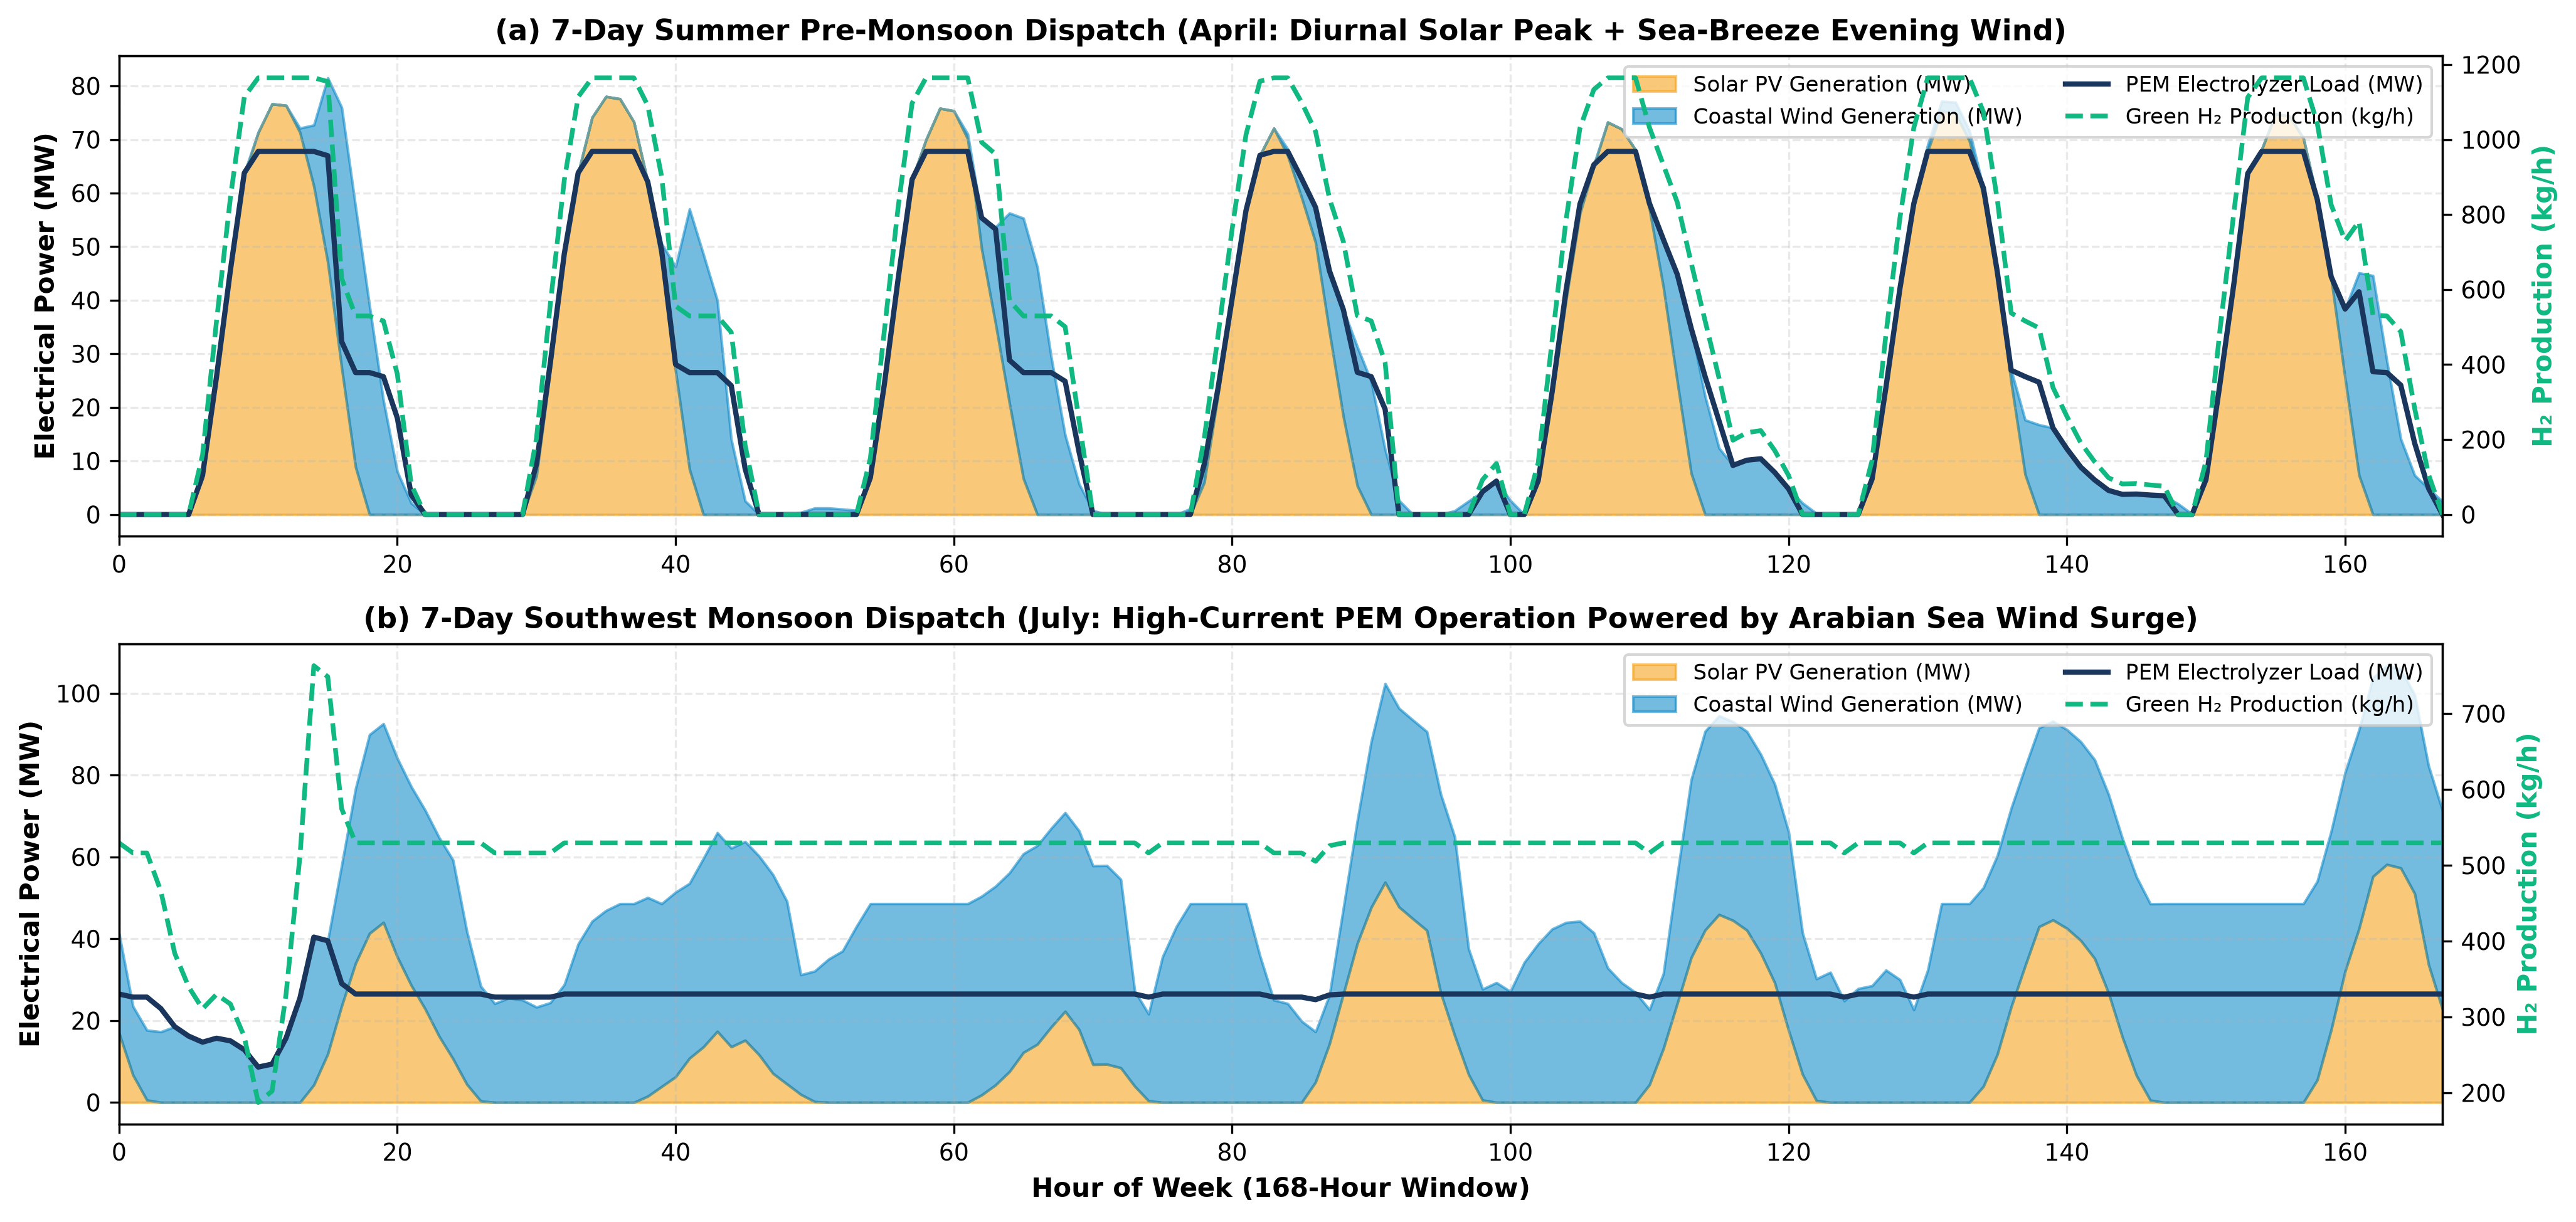
\includegraphics[width=\columnwidth]{figures/fig6_dynamic_dispatch_monsoon_vs_summer.png}
\caption{Hourly dynamic dispatch verification ($168\text{ h}$) of the NSGA-II Knee-Point plant: (a) Pre-monsoon summer week (April, solar-dominant diurnal high-current ramping); (b) Southwest Monsoon week (July, continuous wind-dominant baseload operation); (c) Pressurized $\text{H}_2$ buffer tank inventory ($14,000\text{ kg}$ capacity) and $\text{LiFePO}_4$ state of charge.}
\label{fig:dispatch}
\end{figure}

\section{Conclusion}
This paper presented an integrated Process Systems Engineering, coastal infrastructure siting, and Green Artificial Intelligence framework for the optimal synthesis and online fault monitoring of a $500\text{ kg H}_2/\text{h}$ coastal hybrid Wind--Solar--Battery--PEM green hydrogen plant in the Manipal--Mangalore industrial corridor. Key conclusions include:
\begin{enumerate}
    \item Operating a $38.98\text{ MW}$ nominal PEMWE stack dynamically up to $i_{\max}^* = 2.84\text{ A/cm}^2$ enables absorption of $67.78\text{ MW}$ renewable peaks, saving over $\text{INR } 167\text{ Cr}$ in stack CAPEX while preserving a $10.83$-year stack lifetime ($\dot{V}_{\text{deg}} = 1.898\ \mu\text{V/h}$).
    \item Embedding dimensionless electrochemical-dispatch invariants into the proposed \texttt{Green-MLP} surrogate reduces trainable parameters by $98.88\%$ ($4,900$ vs.\ $438,468$) and compute energy by $99.38\%$ while achieving $R^2 = 0.9984$ and a $10,592\times$ speedup over $8,760$-hour DAE simulation.
    \item Multi-objective NSGA-II optimization exploiting coastal Karnataka wind--solar complementarity achieves an LCOH of $\text{INR } 296.70/\text{kg H}_2$ (\$$3.53/\text{kg}$), $\text{LPSP} = 0.94\%$, and lifecycle carbon intensity of $2.203\text{ kg CO}_2\text{e/kg H}_2$, reducing LCOH by $9.79\%$ and $21.60\%$ compared to wind-only and solar-only baselines.
    \item Online PCA $T^2$ and Jackson--Mudholkar $Q$ monitoring decouples renewable load swings from internal stack degradation, delivering a $52$-hour early detection lead time for incipient membrane dehydration ($91.82\%$ FDR) and $100.0\%$ detection of high-current anodic flooding ($\text{FAR} = 1.86\%$).
\end{enumerate}

\section*{Acknowledgment}
The authors thank the Department of Computer Science and Engineering, the Department of Civil Engineering (School of Civil \& Chemical Engineering), and the IIChE Student Chapter at Manipal Institute of Technology (MIT), Manipal Academy of Higher Education (MAHE), for providing computational resources and technical inspiration under CHEMIGNITE 2026 (ASPIRE).

\begin{thebibliography}{99}

\bibitem{pujari2026}
N. K. Pujari, R. K. Inapakurthi, and K. Mitra, ``Integrated forecasting and design of distributed wind-to-hydrogen systems for urban sustainability,'' \emph{Comput. Chem. Eng.}, vol. 211, p. 108842, Aug. 2026.

\bibitem{masampally2026}
V. S. Masampally, K. Mitra, and V. Runkana, ``Modeling and simulation of hydrogen production in a PEM water electrolyzer at high current densities,'' \emph{Energy Convers. Manag.}, vol. 352, p. 121110, 2026.

\bibitem{mitra2025book}
K. Mitra, R. Everson, and J. Fieldsend, Eds., \emph{Optimization, Uncertainty and Machine Learning in Wind Energy Conversion Systems}. Cham, Switzerland: Springer Nature, Jan. 2025.

\bibitem{inapakurthi2025}
R. K. Inapakurthi, N. K. Pujari, and K. Mitra, ``Maximizing energy production from wind farm layout using model predictive control,'' in \emph{Optimization, Uncertainty and Machine Learning in Wind Energy Conversion Systems}, K. Mitra \emph{et al.}, Eds. Cham: Springer, 2025, pp. 85--112.

\bibitem{abhishek2025}
Abhishek, N. K. Pujari, and K. Mitra, ``AI-driven wind resource modelling for efficient wind-to-hydrogen system design at Jaisalmer,'' in \emph{Proc. Int. Conf. AI Manuf. Sustain. (AIMS)}, Dec. 2025, pp. 1--8.

\bibitem{madakyaru2024}
M. Madakyaru, C. N. Bhushan, and S. R. Kulkarni, ``Multivariate statistical process monitoring and improved latent-variable fault detection for nonlinear chemical processes,'' \emph{J. Process Control}, vol. 134, p. 103148, 2024.

\bibitem{nounou2012}
M. N. Nounou, B. R. Bakshi, P. K. Goel, and X. Shen, ``ches-PCA and multiscale latent variable modeling for fault detection in dynamic chemical systems,'' \emph{AIChE J.}, vol. 48, no. 8, pp. 1775--1793, 2002.

\bibitem{jackson1979}
J. E. Jackson and G. S. Mudholkar, ``Control procedures for residuals associated with principal component analysis,'' \emph{Technometrics}, vol. 21, no. 3, pp. 341--349, Aug. 1979.

\bibitem{deb2002}
K. Deb, A. Pratap, S. Agarwal, and T. Meyarivan, ``A fast and elitist multiobjective genetic algorithm: NSGA-II,'' \emph{IEEE Trans. Evol. Comput.}, vol. 6, no. 2, pp. 182--197, Apr. 2002.

\bibitem{schwartz2020}
R. Schwartz, J. Dodge, N. A. Smith, and O. Etzioni, ``Green AI,'' \emph{Commun. ACM}, vol. 63, no. 12, pp. 54--63, Dec. 2020.

\bibitem{raissi2019}
M. Raissi, P. Perdikaris, and G. E. Karniadakis, ``Physics-informed neural networks: A deep learning framework for solving forward and inverse problems involving nonlinear partial differential equations,'' \emph{J. Comput. Phys.}, vol. 378, pp. 686--707, Feb. 2019.

\bibitem{springer1991}
T. E. Springer, T. A. Zawodzinski, and S. Gottesfeld, ``Polymer electrolyte fuel cell model,'' \emph{J. Electrochem. Soc.}, vol. 138, no. 8, pp. 2334--2342, Aug. 1991.

\bibitem{carmo2013}
M. Carmo, D. L. Fritz, J. Mergel, and D. Stolten, ``A comprehensive review on PEM water electrolysis,'' \emph{Int. J. Hydrogen Energy}, vol. 38, no. 12, pp. 4901--4934, Apr. 2013.

\bibitem{liso2018}
V. Liso, G. Savoia, S. S. Araya, G. Cinti, and S. K. Kær, ``Modelling and experimental analysis of a polymer electrolyte membrane water electrolyzer cell at different operating temperatures,'' \emph{Energies}, vol. 11, no. 12, p. 3273, Nov. 2018.

\bibitem{siracusano2017}
S. Siracusano, N. Van Dijk, R. Backhouse, L. Merlo, V. Baglio, and A. S. Aric\`o, ``Degradation issues of PEM electrolysis MEAs,'' \emph{Renew. Energy}, vol. 123, pp. 52--57, Aug. 2018.

\bibitem{qin2012}
S. J. Qin, ``Survey on data-driven industrial process monitoring and diagnosis,'' \emph{Annu. Rev. Control}, vol. 36, no. 2, pp. 220--234, Dec. 2012.

\bibitem{gupta2021}
R. Gupta \emph{et al.}, ``GIS and machine learning-assisted spatial scenario modeling for sustainable infrastructure and resource management,'' \emph{Sustain. Cities Soc.}, vol. 74, p. 103195, Nov. 2021.

\bibitem{mnre2023}
Ministry of New and Renewable Energy (MNRE), \emph{National Green Hydrogen Mission}. New Delhi, India: Government of India, Jan. 2023.

\bibitem{nasapower2026}
NASA POWER Project, ``Prediction Of Worldwide Energy Resources (Agroclimatology \& Renewable Energy Hourly Archive, Coastal Karnataka Grid $13.3525^\circ\text{N}, 74.7928^\circ\text{E}$),'' National Aeronautics and Space Administration, Hampton, VA, USA, 2026.

\end{thebibliography}

\end{document}
